\documentclass[times,specification,annotation]{itmo-student-thesis}

\usepackage{icomma}
\usepackage{tikz}
\usetikzlibrary{arrows}
\usepackage{filecontents}
\usepackage{rotating}

\addbibresource{bachelor-thesis-kate.bib}

\newcommand{\specialcell}[2][c]{%
  \begin{tabular}[#1]{@{}c@{}}#2\end{tabular}}
\newcommand{\specialcelll}[2][l]{%
  \begin{tabular}[#1]{@{}l@{}}#2\end{tabular}}

\begin{document}

\studygroup{P3420}
\title{Автоматическое выделение функциональных наборов генов в базе GEO с помощью дифференциальной экспрессии}
\author{Беляева Екатерина Сергеевна}{Беляева Е.С.}
\supervisor{Сергушичев Алексей Александрович}{Сергушичев А.А.}{к.т.н.}{доцент кафедры КТ}
\publishyear{2018}
\startdate{01}{сентября}{2017}
\finishdate{31}{мая}{2018}
\defencedate{19}{июня}{2018}

\secretary{Бутько Е.Ф.}

%% Задание
%%% Техническое задание и исходные данные к работе
\technicalspec{В рамках выпускной квалификационной работы основной задачей является построение функциональных наборов генов из базы GEO с помощью анализа дифференциальной экспрессии, а также обеспечение интерфейса доступа к ним}

%%% Содержание выпускной квалификационной работы (перечень подлежащих разработке вопросов)
\plannedcontents{\begin{enumerate}
    \item Обзор предметной области.
    \item Анализ существующих сервисов.
    \item Загрузка данных и их обработка.
    \item Построение модулей генов при помощи анализа дифференциальной экспрессии.
    \item Обеспечение интерфейса доступа к модулям генов.
    \item Анализ полученных результатов.
\end{enumerate}}

%%% Исходные материалы и пособия 
\plannedsources{\begin{enumerate}
    \item Bioconductor. Bioconductor is an open source, open development software project to provide tools for the analysis and comprehension of high-thoughput genomic data. [Электронный ресурс]. URL: https://www.bioconductor.org/;
    \item Docker. Docker is the software container platform. [Электронный ресурс]. URL: https://www.docker.com/;
    \item Терри А.Браун Геномы / Терри А.Браун. - М.-Ижевск: Институт компьютерных исследований, 2011. - 921 c.  
\end{enumerate}}

%%% Цель исследования
\researchaim{Получить новую базу функциональных наборов генов.}

%%% Задачи, решаемые в ВКР
\researchtargets{\begin{enumerate}  
    \item изучение существующих сервисов для работы с данными экспрессии генов;
    \item построение новых функциональных наборов генов из базы GEO при помощи анализа дифференциальной экспрессии;
    \item анализ полученных результатов;
    \item обеспечение интерфейса доступа к модулям генов.
\end{enumerate}}

%%% Использование современных пакетов компьютерных программ и технологий
\addstage{R (библиотеки GEOquery, limma, dplyr, stringr, data.table, magrittr, tibble)}{Глава 2, Глава 3}
\addstage{Python 2,3 (библиотеки pandas, subprocess, re, csv)}{Глава 2, Глава 4}
\addstage{Bash}{Глава 2}
\addstage{Kotlin}{Глава 2, Глава 4}
\addstage{Django}{Глава 2, Глава 4}
\addstage{Java Script}{Глава 2, Глава 4}
\addstage{React}{Глава 2, Глава 4}
\addstage{HTML}{Глава 2, Глава 4}
\addstage{CSS}{Глава 2, Глава 4}
\addstage{Docker}{Глава 2, Глава 4}

%%% Краткая характеристика полученных результатов 
\researchsummary{По итогу работы был реализован сервис с возможностью предоставления доступа к модулям генов конечному потребителю.}

%%% Гранты, полученные при выполнении работы 
\researchfunding{Грантов или других форм государственной поддержи и субсидирования в процессе работы не предусматривалось.}

%%% Наличие публикаций и выступлений на конференциях по теме выпускной работы
\researchpublications{Публикаций и выступлений на конференциях не было.}

\maketitle{Бакалавр}

%% Оглавление
\tableofcontents

%% Введение
\startprefacepage

Жизнь, какой мы ее видим, создается геномами мириад организмов, с которыми мы делим нашу планету. Каждый из этих организмов обладает геномом, содержащем биологическую информацию, необходимую для построения и поддержания организма живущего в настоящий момент времени представителя данного вида.\cite{Introduction} Биоинформатика ~-- наука, стоящая на границе биологии и информатики, активно развивается в течении последних десятилетий. Открываются новые направления исследований, появляется всё больше данных, в том числе и открытых.

Одним из направлений биоинформатики являются исследования, связанные с экспрессией генов, т.е. с процессом преобразования последовательности гена в функциональный продукт (обычно белок). Существует множество связанных с этим данных. Самой известной и часто используемой базой данных экспрессии генов является база данных ​Gene Expression Omnibus (GEO). Она открытая, и именно она и будет использована в дальнейшей работе. 

Есть множество сервисов, работающих с данными экспрессии генов. В этой работе был рассмотрен и расширен сервис GeneQuery, который является поисковым порталом, использующим данные из базы GEO. Сервис плохо работал с маленькими по числу образцов датасетами, следовательно существовала проблема изменения принципа обработки данных. Так, целью данной бакалаврской работы являлось построение функциональных наборов генов из базы GEO с помощью дифференциальной экспрессии. Сервис GeneQuery был расширен для поддержки новых данных. Ожидается, что используя новую базу функциональных групп генов может быть выявлена потенциально значимая биологическая информация, а сам сервис может быть использован исследователями в области биоинформатики.        

%% Содержательная часть.
\chapter{Обзор предметной области}

\section{Основные понятия и определения}
\startrelatedwork
\textit{Биоинформатика} ~-- это междисциплинарная область, работающая с биологическими данными. Она сочетает в себе информатику, биологию, математику, статистику и ещё множество областей. Также широк и круг исследований биоинформатики, однако данная работа будет сосредоточена на таком направлении, как экспрессия генов.

\textit{Ген} ~-- единица наследственности живых организмов.

\textit{Экспрессия гена} ~-- процесс преобразования последовательности гена в функциональный продукт (обычно белок). Она может быть измерена количественно. 

\textit{Дифференциальная экспрессия гена} ~-- изменение уровня экспрессии гена в зависимости от биологического состояния.

\textit{Функциональная группа генов} ~-- отвечает за конкретное биологическое явление или несколько явлений. 

Для примера можно рассмотреть гликолиз ~-- процесс расщепления глюкозы в клетках, сопровождающийся синтезом АТФ. Для протекания этого процесса необходимы ферменты, т.е. ускорители химических реакций. В гликолизе участвуют ферменты гексокиназа, глюкозофосфатизомераза, енолаза и другие. Их структуры определяются генами HK1, PGI1, ENO1 и т.д.\cite{Glycolysis} Все эти гены являются функциональной группой генов для процесса гликолиз.

\section{База данных GEO}

Биоинформатика обладает большим объемом информации, который нужно где-то хранить. Для этой цели существуют множество баз данных. Накопление данных о генах, проявивших себя в биологических экспериментах, т.е. функциональных групп генов, является важной задачей потому, что эта информация может быть полезна в будущем. Самым известным открытым репозиторием для хранения данных экспрессии генов является \textit{Gene Expression Omnibus}. Или же сокращенно \textit{GEO}.

Проект GEO был инициирован в ответ на растущую потребность в общедоступном хранилище данных экспрессии генов.\cite{GEO} Эксперименты, хранящиеся в репозитории, имеют определенную структуру. Для каждого эксперимента представлены: 
\begin{itemize}
    \item GSM (Geo SaMple) ~-- \textit{образцы} или \textit{сэмплы} ~-- эти данные содержат информацию об организмах, участвовавших в эксперименте, об условиях эксперимента.
    \item GSE (Geo SEries) ~-- \textit{серия} ~-- объединяет в себе несколько образцов и хранит данные о числовых значениях экспрессии генов каждого образца. Как правило это ~20000 генов на каждый обзазец.
    \item GPL (Geo PLatform) ~-- \textit{платформа}, на которой вычислялась экспрессия. Важным компонентом, хранящимся здесь, является информация для каждого гена о соответствии его entrez к symbol.     
\end{itemize}

Количество данных GEO огромно и постоянно растет, в следствии чего база представляет исключительный интерес в биоинформатическом сообществе. Как было отмечено ранее, данная работа посвящена обработке данных именно из GEO.   

\section{Сервис GeneQuery}

Проект GeneQuery\cite{GeneQuery} - это поисковый портал, основанный на автоматическом выделении наборов генов с помощью кластеризации. Работает с данными экспрессии генов из базы данных GEO для организмов Homo Sapience, Mus Musculus и Rattus Norvegicus, т.е. с человеком, мышью и крысой. 

GeneQuery имеит такие достоинства, как высокая скорость обновления данных (новые данные из GEO можно портировать в GeneQuery), быстрая скорость выдачи результата для пользователя, простота использования. Сервис достаточно хорошо работает для средних по размеру датасетов (по числу образцов), но не подходит для маленьких. Для последних можно использовать анализ дифференциальной экспрессии, что и сделано в альтернативной версии GeneQuery - в GeneQueryDE. 

\section{Цель и актуальность работы}

Целью данной работы являлось построение наборов генов по экспериментам из базы GEO c помощью анализа дифференциальной экспрессии и обеспечение интерфейса доступа к ним. 

Портал GeneQuery расширен для поддержки новых данных до версии GeneQueryDE. Сервис может быть использован исследователями в области биоинформатики. Ожидается, что используя новую базу функциональных групп генов может быть выявлена потенциально значимая биологическая информация. 

\chapterconclusion

В данной главе был произведен обзор предметной области. А именно, рассмотрены основные понятия, являющиеся базовыми для понимания дальнейших действий. Рассмотрены сервисы, на которых строится данная работа, а также обозначены её цель и значимость. 
\finishrelatedwork

\chapter{Схема сервиса}

Взаимодействие элементов системы представлено на рисунке~\ref{service}. 

\begin{figure}[!h]
    \caption{Схема сервиса.}\label{service}
    \centering
    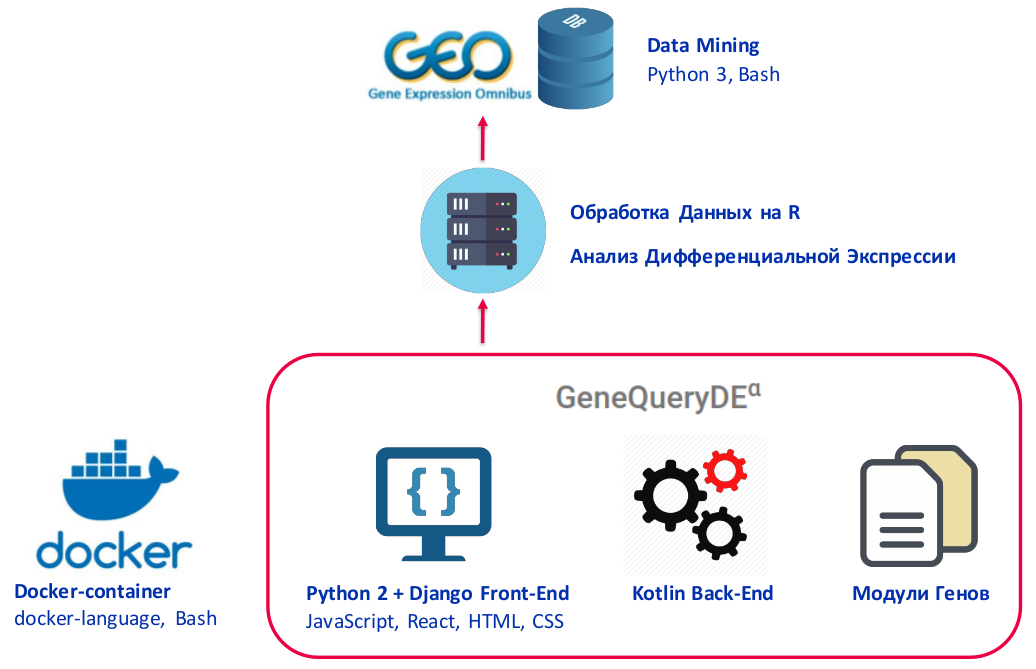
\includegraphics[width=0.9\textwidth]{service_scheme.png}
\end{figure}

С начала данные были загружены из базы GEO на сервер. Для этого использовались языки Python 3 и Bash. Далее на сервере происходила их обработка, и при помощи анализа дифференциальной экспрессии строились модули генов. Для этого использовался язык R. Bioconductor ~-- это проект на R, содержащий множество библиотек для анализа геномных данных.\cite{Bioconductor}. В том числе имеет библиотеку для взаимодействия с базой данных GEO. Так, работая на R, были использованы пакеты GEOquery и limma. 

После того, как модули генов были построены, сервис GeneQuery был расширен для поддержки новых данных до версии GeneQueryDE. Сам сервис состоит из двух репозиториев - front-end части на Python 2 + Django и back-end части на Kotlin. После, GeneQueryDE с новыми данными был упакован в docker-контейнер и запущен. Сейчас сервис доступен по адресу \textit{http://genome.ifmo.ru/genequery-de}.

\chapterconclusion

В данной главе была представлена схема работы системы и описаны основные использованные технологии.

\chapter{Построение модулей генов}

\section{Загрузка данных}

База данных GEO имеет сложную структуру. Например, датасет GSE40554-GPL4125 находится по адресу \textit{https://ftp.ncbi.nlm.nih.gov/geo/series/GSE40nnn/GSE40554/matrix/GSE40554-GPL4125\_series\_matrix.txt.gz}, а аннотация к нему лежит на \textit{https://ftp.ncbi.nlm.nih.gov/geo/platforms/GPL4nnn/GPL4125/annot/} \textit{GPL4125.annot.gz}. При скачивании данных, структура GEO была сохранена. 

\begin{lstlisting}[float=!h, caption={Загрузка данных из GEO.}, captionpos=b, label={downloadGEO}, basicstyle=\footnotesize, language=Python]
import subprocess
import csv

def download_data(file_name, kind_data): 
    with open(file_name,'r') as tsvin:
        tsvin = csv.reader(tsvin, delimiter='\t')
        indexes = []
        
        for (i, row) in enumerate(tsvin):
            if i == 0:
                if kind_data == 'series':
                    indexes = [row.index(j) for j in ['Series', 'Series_url']]
                else:
                    indexes = [row.index(j) for j in ['Platforms', 'Platforms_url']]
            else:    
                try:
                    dif_string = 'https://ftp.ncbi.nlm.nih.gov/'
                    path = row[indexes[1]].replace(dif_string, '')
                    path = path[:(path.rindex('/')+1)]
                    directory = "../" + path

                    subprocess.call(["mkdir", "-p", directory])
                    subprocess.call(["wget", "-c", "-P", directory, row[indexes[1]]])

                except:
                    pass

\end{lstlisting}


Основная функция загрузки приведена на листинге~\ref{downloadGEO}. Всего было загружено 74177 датасетов типа GSE (с экспрессией генов) и 790 GPL (аннотаций) для видов Homo Sapience, Mus Musculus и Rattus Norvegicus. Далее GSE были сопоставлены с аннотациями и выяснилось, что 29098 датасетов пригодно для построения таблиц ​дифференциальной экспрессии.


\section{Автоматическая обработка}

После получения таблицы с матчингом GSE с GPL, для каждого эксперимента надо было построить модули генов с применением анализа дифференциальной экспрессии. Для этого, для каждого датасета были выполнены действия:
\begin{itemize}
    \item Выявлены уникальные условия каждого эксперимента.
    \item Соотнесены гены с аннотациями к ним.
    \item Нормализованны данные.
    \item Построены пары условий.
    \item Построены таблицы дифференциальной экспрессии.
\end{itemize}

\subsection{Выявление уникальных условий каждого эксперимента}

GSE датасет содержит таблицу с указанием информации по каждому образцу, участвовавшему в эксперименте. В том числе, содержатся условия эксперимента для каждого образца. Эти данные записаны в столбцах <<charactericstics>>, которых может быть от 1 до n. Требовалось автоматически выделять биологические состояния.  

Поиск нужных для парсинга столбцов на листинге~\ref{searchCharacteristicsColumns}. 

\begin{lstlisting}[float=!h, caption={Поиск столбцов <<charactericstics>>.}, captionpos=b, label={searchCharacteristicsColumns}, basicstyle=\footnotesize, language=R]

getCharacteristicsColumns <- function(gse) {
  col <- colnames(pData(gse))
  characteristics <- c()
  for (ch in col) {
    if (grepl("characteristics", ch)) characteristics <- c(characteristics, ch)
  }
  return(characteristics)
}

\end{lstlisting}

Как можно видеть на листинге~\ref{fillGseConditionColumn}, возможна ситуация, когда уникальные состояния выделить не удавалось. Это могло быть связано с пропусками данных в столбцах <<charactericstics>> или же с тем, что условия не несли в себе универсального значения. Например, в датасете, состоящем из восьми образцов, в одной из колонок <<charactericstics>> могли быть написаны цифры от 1 до 8, соответствующие просто номерам образцов. Такие случаи игнорировались и не участвовали в дальнейшем анализе.  

\begin{lstlisting}[float=!h, caption={Выделение условий.}, captionpos=b, label={fillGseConditionColumn}, basicstyle=\footnotesize, language=R]

characteristics <- getCharacteristicsColumns(gse)
conditionLists <- list()

...

if (length(characteristics) > 0) {
    message("There are characteristics columns in the samples table.")
    conStructure <- getConditionsFromCharacteristics(gse, characteristics)
    conditionLists <- conStructure$conditionsList
    explanatoryTable <- conStructure$explanatoryTable 
  }
  
  if (length(conditionLists) > 0 && length(unique(unlist(conditionLists))) > 1) {
    pData(gse)$condition <- fillGseConditionColumn(conditionLists) 
    ...

  } else 
    message("Characteristics columns in the samples table don't exist or were unhelpful.")

\end{lstlisting}

\subsection{Соотнесение генов и аннотаций}
Требовалось соотнести entrez генов из таблицы с экспрессией с их symbol из таблицы с аннотацией. При построении модулей дифференциальной экспрессии колонка с названиями генов также была сохранена в таблице.

\begin{lstlisting}[float=!h, caption={Выделение 7000 генов с максимальной экспрессией.}, captionpos=b, label={get7000}, basicstyle=\footnotesize, language=R]
collapseData <- function(gse, gpl, FUN=median) {
  ranks <- apply(exprs(gse), 1, FUN)
  ranks <- data.frame(r = ranks, i = seq_along(ranks))
  table <- inner_join(rownames_to_column(gpl), rownames_to_column(ranks), 
           by="rowname") %>% 
           mutate(j = seq_along(symbol))
  t <- table[order(table$r, decreasing=T), ][1:7000,]
  keep <- t$i
  res <- gse[keep, ]
  rownames(res) <- table$ENTREZ_GENE_ID[t$j]
  fData(res)$symbol <- t$symbol
  return(res)
}

...

gpl <- createGenesSymbolsTable(gpl)
es <- collapseData(gse, gpl)

\end{lstlisting} 

На листинге~\ref{get7000} происходит матчинг entrez генов с их symbol, выделяются 7000 генов с наибольшей экспрессией. На основе этого набора генов в дальнейшем строются модули с дифференциальной экспрессией.    

\subsection{Нормализация данных}

В процессе обработки данных были совершены следующие действия:
\begin{itemize}
    \item Убраны дублирующиеся данные​.
    \item Убраны данные с пропусками​.
    \item Отобраны 7000 генов с самой высокой экспрессией​ (листинг~\ref{get7000}).
    \item Логарифмизация данных при большом размахе значений экспрессии (листинг~\ref{normalizeData}).
\end{itemize}

\begin{lstlisting}[float=!h, caption={Логарифмизация данных.}, captionpos=b, label={normalizeData}, basicstyle=\footnotesize, language=R]

if (max(exprs(es)) - min(exprs(es)) > 100)
        exprs(es) <- normalizeBetweenArrays(log2(exprs(es)+1), method="quantile")

\end{lstlisting} 

Как правило, после удаления дублирующихся данных и данных с пропусками в рассмотрении оставался набор, состоящий примерно из 20000 генов.

\subsection{Построение пар условий}

Так как дифференциальная экспрессия ~-- это изменение активности гена в зависимости от конкретного биологического состояния, то на данном этапе требовалось составить пары условий с различием в одно состояние. Для этого обрабатывался столбец \textit{pData(gse)\$condition}, получение которого показано на листинге~\ref{fillGseConditionColumn}.

\subsection{Построение таблиц дифференциальной экспрессии}

Для каждой пары условий, полученной по результатам предыдущего пункта, требовалось построить таблицу с дифференциальной экспрессией. Построение показано на листинге~\ref{fitLinearModel}.

\begin{lstlisting}[float=!h, caption={Построение модулей генов при помощи дифференциальной экспрессии.}, captionpos=b, label={fitLinearModel}, basicstyle=\footnotesize, language=R]

fitLinearModel <- function(fit, conditions, design, deSize) {
  deList <- list()
  for (i in 1:length(conditions)) {
    
    contrasts <- makeContrasts2(
               c("condition", conditions[[i]]$firstCon, conditions[[i]]$secondCon), 
               levels=design)
    
    fit2 <- contrasts.fit(fit, contrasts)
    
    df.residual <- unique(fit2$df.residual)
    if ((length(df.residual) == 1 && df.residual[1] != 0) ||
        (length(df.residual) != 1)) {
      
      fit2 <- eBayes(fit2)
      
      deList[[i]] <- data.table(
        topTable(fit2, adjust.method="BH", number=deSize, sort.by = "B"), 
        keep.rownames = T)
    }
  }
  return(deList)
}

\end{lstlisting} 

Пример таблицы приведен на рисунке~\ref{difExprs}. Модуль содержит 7000 генов и включает в себя информацию о entrez гена, его названии, средней экспрессии и различные статистические метрики. 

Модули получилось построить для 16246 экспериментов.

\begin{figure}[!h]
    \caption{Таблица дифференциальной экспрессии генов.}\label{difExprs}
    \centering
    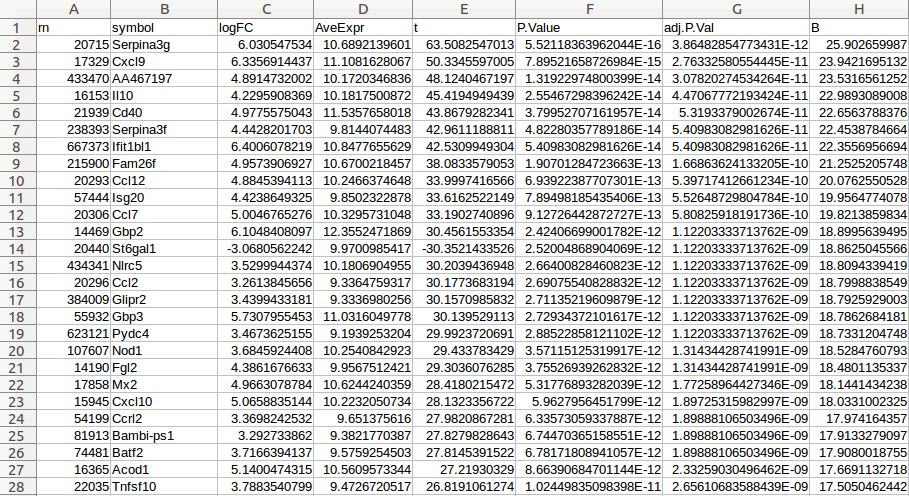
\includegraphics[width=1\textwidth]{difExprs.jpg}
\end{figure}

\section{Верхняя и нижняя регуляции генов}

Верхняя и нижняя регуляция генов ~-- это сравнение их активностей относительно друг друга. На предыдущем этапе были постоены таблицы генов при противопоставлении двух разных биологических состояний. Так, на данном этапе для каждого из модулей дифференциальной экспрессии генов требовалось построить дескриптивную выборку. По максимальному значению t-статистики отбиралось 200 генов, что соответствует верхней регуляции и по минимальному значению t-статистики отбиралось 200 генов, соответствующих нижней регуляции. Полученные модули сохранялись. Также на их основе строились \textit{.gmt} файлы для каждого вида (человек, мышь, крыса). Файлы содержали гены из экспериментов. А именно, для каждого эксперимента было представленно название, универсум (7000 генов), название модулей и соответствующие выборки по 200 генов.

По итогам выборак по 200 генов, всего было получено 851396 новых модулей, которые затем были встроены в обработку сервиса GeneQueryDE.

\chapterconclusion

В данной главе был описан основной этап работы, который заключался в загрузке данных из базы GEO и построении модулей генов. Приведены цифры обработки данных и итоговые результаты.  


\chapter{Обеспечение интерфейса доступа к данным}

После получения модулей генов и \textit{.gmt} файлов требовалось расширить сервис GeneQuery для возможности работы с новыми данными. Так была создана версия проекта GeneQueryDE. 

\section{Метод поиска модулей генов}

GeneQueryDE со стороны пользователя принимает название организма и некий набор генов. Затем на основании статистической значимости выдаются подобранные модули. Для этого отдельно оценивается значимость каждого модуля, используя тест Фишера. При этом обозначаются две гипотезы:
\begin{itemize}
    \item \textit{нулевая} ~-- связи между двумя наборами генов нет, пересечение случайно.
    \item \textit{альтернативная} ~-- пересечение получено не случайно, наблюдается статистически значимая связь, гены связанны одним процессом.
\end{itemize}

\begin{table}[!h]
    \caption{Тест Фишера}\label{fisherTable}
    \centering
    \begin{tabu}{ |X[l]|*{3}{X[c]|}}
        \hline
         & в запросе & вне запроса & \cellcolor{Gray} всего\strut\\ \hline
        в модуле & a & b & \cellcolor{Gray} a + b\\ \hline
        не в модуле & c & d & \cellcolor{Gray} c + d\\ \hline
        \cellcolor{Gray} всего & \cellcolor{Gray} a + c & \cellcolor{Gray} b + d & \cellcolor{Gray} n\\ \hline
    \end{tabu}
\end{table}

, где \textit{a, b, c, d} - количества генов в соответствующих категориях​;

\textit{n} - размер универсума (= 7000 генов)

\begin{equation}
\label{pvalue}
    p = \binom{a+b}{a}\binom{c + d}{c}/\binom{n}{a+c} = \frac{(a+b)!(c+d)!(a+c)!(b+d)!}{n!a!b!c!d!}
\end{equation}

Используя формулу~\ref{pvalue} производится расчет таблицы~\ref{fisherTable}. Чем меньше полученное \textit{p-value}, тем значимее модуль. Таким образом, число выражает нашу <<неуверенность>> в связи модуля и запроса. 

Далее происходит корректировка на множественные сравнения. Для этого применяется поправка Бонферрони\cite{Bonferroni} ~-- полученное \textit{p-value} умножается на количество модулей, т.е. на число произведенных сравнений. Полученное значение после поправки, \textit{adj.p-value}, равно вероятности отклонить хотя бы одну нулевую гипотезу из всех проверенных, т.е. вероятности совершить хотя бы одну ошибку первого рода. Если \textit{adj.p-value ≤ 0.01}, то модуль признается статистически значимым и выводится в качестве результата запроса.

\section{Представление результатов пользователю}

Пользователь выбирает организм и вводит соответствующий ему набор генов, как показано на рисунке~\ref{clientRequest}. Система выдает ответ в виде статистически значимых модулей (рисунок~\ref{clientResponse}), в которых найдены совпадающие гены. Список отсортирован в порядке возрастания логарифма \textit{adj.p-value ≤ 0.01}. Как можно видеть, информация, которую получает пользователь по каждому модулю, также включает в себя название эксперимента, название модуля, число перекрытий генов, ссылку на эксперимент и возможность загрузки таблицы с дифференциальной экспрессией данного модуля.

\begin{figure}[!h]
    \caption{Запрос.}\label{clientRequest}
    \centering
    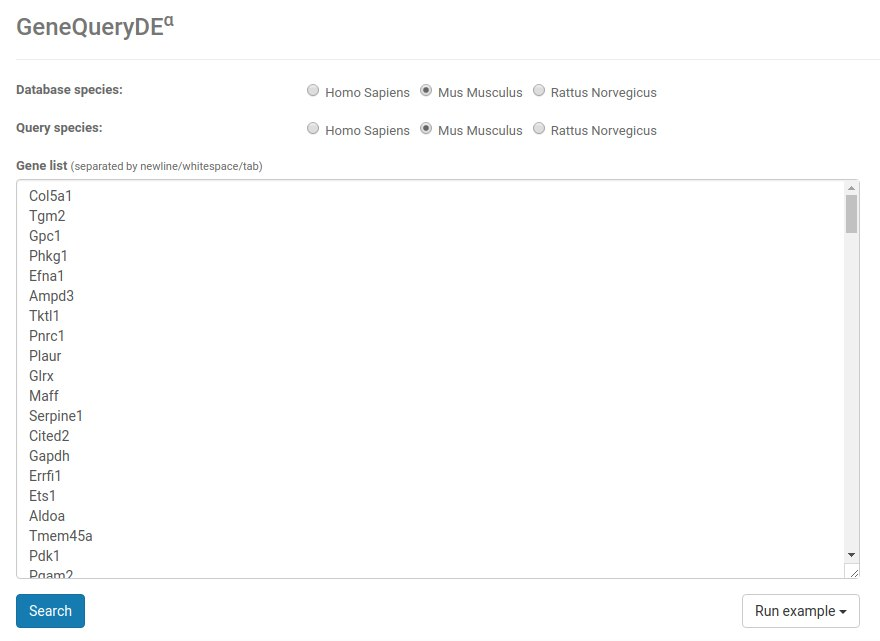
\includegraphics[width=0.9\textwidth]{request.jpg}
\end{figure}

\begin{figure}[!h]
    \caption{Результат запроса.}\label{clientResponse}
    \centering
    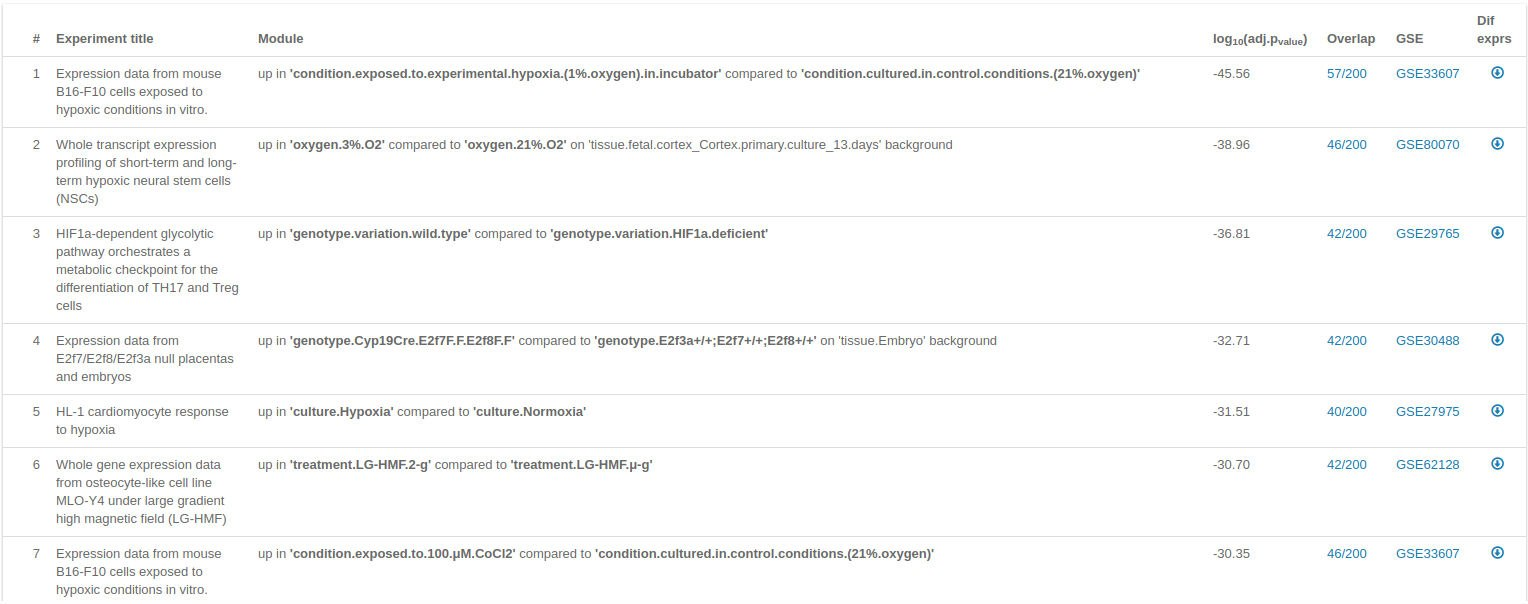
\includegraphics[width=1\textwidth]{response.jpg}
\end{figure}

Название модуля включает в себя два биологических состояния, на основании которых была вычисленна дифференциальная экспрессия, и условия, которые не менялись.

Например, \textit{up in} \textbf{\lq oxygen.3\%.O2\rq } \textit{compared to} \textbf{\lq oxygen.21\%.O2\rq} \textit{on \lq tissue.fetal.cortex\_Cortex.primary.culture\_13.days\rq~background} ~-- ответ на гипоксию. Здесь гены при \textbf{\lq oxygen.3\%.O2\rq} реагируют против \textbf{\lq oxygen.21\%.O2\rq} на основании условий, присутствующих в обоих экспериментах. 

\section{Контейнеризация}

В соответствии с документацией docker\cite{Docker} был создан Dockerfile для построения образа и впоследующем контейнера с сервисом. Используя данную технологию, проект GeneQueryDE, состоящий из front-end и back-end частей был упакован в docker-контейнер с доступом к данным с сервера ~-- к модулям генов и \textit{.gmt} файлам. Контейнер запущен, т.ч. сервис доступен по адресу \textit{http://genome.ifmo.ru/genequery-de}.  

\chapterconclusion

В данной главе был описан интерфейс сервиса GeneQueryDE, способ выдачи результата и пример запроса-ответа. Также сказано о возможности доступа к сервису посредством интернета. 

\chapter{Сравнение и анализ результата}

\section{Сравнение GeneQuery с GeneQueryDE по числу данных}

На рисунке~\ref{GSEnumbers} представленно сравнение сервисов по количеству пар GSE+GPL, для которых в последствии были построены модули генов. Как можно увидеть, помимо совпадающих экспериментов, проанализированных в обоих сервисах, также много уникальных GSE, обработанных только в одном из проектов. Причем в GeneQueryDE обработано больше. Если для вида Rattus Norvegicus количество уникальных GSE примерно равно в обоих проектах, то, например, для Mus Musculus, сервис GeneQueryDE обрабатывает в 3.15 раза больше данных, чем версия GeneQuery. 

\begin{figure}[!h]
    \caption{Сравнение по парам GSE+GPL.}\label{GSEnumbers}
    \centering
    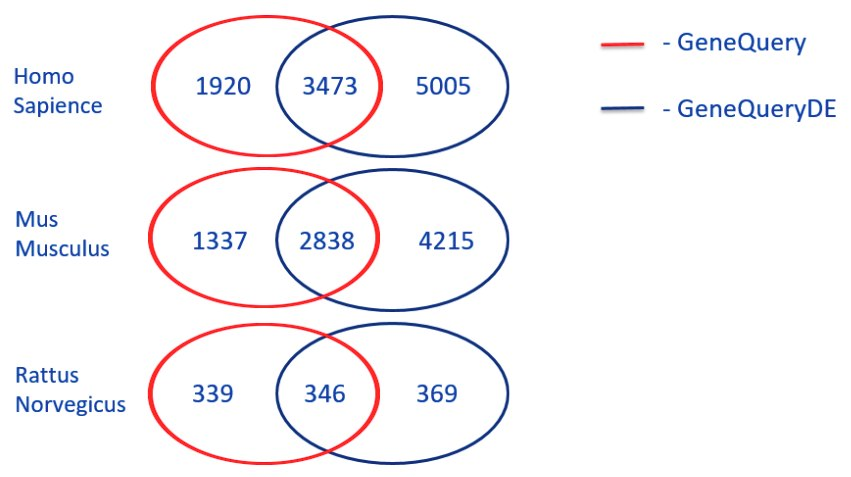
\includegraphics[width=0.8\textwidth]{GSEnumbers.jpg}
\end{figure}

В таблице~\ref{ModulesTable} представлены различия в итоговом числе модулей, полученных для двух сервисов. Видно, что сервис GeneQueryDE работает с гораздо большим количеством данных, чем альтернативная версия.

\begin{table}[!h]
    \caption{Сравнение по модулям генов}\label{ModulesTable}
    \centering
    \begin{tabu}{ |X[l]|*{2}{X[c]|}}
        \cline{2-3}
        \multicolumn{1}{c|}{} & \multicolumn{2}{c|}{Модули экспрессии генов}\\ \cline{2-3}
        \multicolumn{1}{c|}{} & GeneQuery & GeneQueryDE\strut\\ \hline
        Homo Sapience & 117497 & 620216 \\ \hline
        Mus Musculus & 82371 & 213712 \\ \hline 
        Rattus Norvegicus & 13560 & 17468 \\ \hline
    \end{tabu}
\end{table}

\section{Сравнение сервисов}

В данном разделе приведено сравнение существующих проектов с GeneQueryDE. А именно, сервисов GeneQuery, GEOracle\cite{GEOracle}, ARCHS4\cite{ARCHS4} и 
GEO Profiles\cite{GEOprofiles}. Как видно из таблицы~\ref{ServicesTable} все сервисы выполняют разные функции, принимая на вход различные аргументы. Сервис GeneQueryDE делает свою уникальную работу ~-- ищет модули дифференциальной экспрессии генов, перекрывающиеся с запросом пользователя, и выдает их, ранжируя в порядке статистической значимости.

\begin{sidewaystable*}
    \caption{Сравнение сервисов}\label{ServicesTable}
    \centering
    %\begin{tabu}{ |X[l]|*{3}{X[c]|}}
    \begin{tabu}{ |X[l]|m{6.7cm}|m{6.7cm}|m{6.7cm}|}
    \cline{2-4}
        \multicolumn{1}{c|}{} & \cellcolor{Gray} Входные данные & \cellcolor{Gray} Обрабатываемые виды & \cellcolor{Gray} Результаты работы \strut\\ 
        \hline
        \cellcolor{Gray} GeneQuery & Набор генов & \begin{itemize}
            \item Homo Sapience
            \item Mus Musculus
            \item Rattus Norvegicus
        \end{itemize} & \begin{itemize}
            \item Перекрытия генов
            \item Тепловые карты экспрессии генов
        \end{itemize}\\ 
        \hline
        \cellcolor{darkgray} GeneQueryDE & \cellcolor{darkgray} Набор генов & \cellcolor{darkgray} \begin{itemize}
            \item Homo Sapience
            \item Mus Musculus
            \item Rattus Norvegicus
        \end{itemize} & \cellcolor{darkgray} \begin{itemize}
            \item Перекрытия генов
            \item Модули дифференциальной экспрессии
        \end{itemize}\\ 
        \hline 
        \cellcolor{Gray} GEOracle & Набор экспериментов & Без ограничений & \begin{itemize}
            \item Числовые значения дифференциальной экспрессии
            \item Тепловые карты зависимости экспериментов от генов
        \end{itemize}\\ 
        \hline
        \cellcolor{Gray} ARCHS4 & \begin{itemize}
            \item Ген
            \item Набор генов в верхней/нижней регуляции
            \item (доп.параметры: ткани, органы)
        \end{itemize} & \begin{itemize}
            \item Homo Sapience
            \item Mus Musculus
        \end{itemize} & \begin{itemize}
            \item Информация о гене
            \item Средняя экспрессия гена
        \end{itemize}\\ 
        \hline
        \cellcolor{Gray} GEO Profiles & \begin{itemize}
            \item Ген
            \item Эксперимент
            \item Организм
            \item Свободный текст
        \end{itemize} & Без ограничений & \begin{itemize}
            \item Эксперименты с аннотациями
            \item Информация о генах
        \end{itemize}\\ 
        \hline
    \end{tabu}
\end{sidewaystable*}

\chapterconclusion

В данной главе были подведены итоги созданного сервиса GeneQueryDE, а именно произведено его сравнение с альтернативной версией по количеству обрабатываемых данных и сравнение с существующими проектами. 
  

%% Заключение
\startconclusionpage

В результате данной работы:
\begin{itemize}
    \item Построены модули дифференциальной экспрессии генов для видов Homo Sapience, Mus Musculus, Rattus Norvegicus.
    \item Расширен сервис GeneQuery до версии GeneQuery-de, обеспечивающий интерфейс доступа к модулям генов. 
    \item В версии GeneQuery-de значительно увеличено количество обрабатываемых данных по сравнению с GeneQuery. 
    \item Контейнеризация полученного решения.
    \item Сервис GeneQuery-de доступен по ссылке: \textit{http://genome.ifmo.ru/genequery-de}.​
\end{itemize}

\printmainbibliography

\end{document}
